\mcchap{Il portale Covid19-Italy}{cap:portale}
Con il patrocinio dell’Università degli studi dell’Insubria è stato ideato il portale Covid 19-Italy.it\footnote{https://covid19-italy.it}, un sito che permette di visualizzare i dati aggregati e ufficiali sull’andamento della pandemia regione per regione e a livello nazionale, attraverso grafici e confronti.
Sulla pagina principale del sito sono presenti 4 card, che permettono di accedere alle seguenti pagine:
\begin{itemize}
\item \emph{Italy R0(t) Indices} permette di accedere alla pagina sulla stima degli indici di riproduzione R0(t) usando il metodo Wallinga and Teunis, a livello nazionale, regionale e provinciale. (in figura \ref{fig:indici_r0})
\item \emph{Italy dashboard} visualizza il monitoraggio del Covid-19 in Italia, attraverso 9 diversi grafici, sempre aggiornati con la pubblicazione di nuovi dati;
\item \emph{Lombardy dashboard} visualizza l’andamento nella pandemia in dettaglio nella regione Lombardia;
\item \emph{Region dashboard} mostra l’andamento della pandemia in una regione italiana a scelta.
\end{itemize}
\begin{figure}[htp]
    \centering
    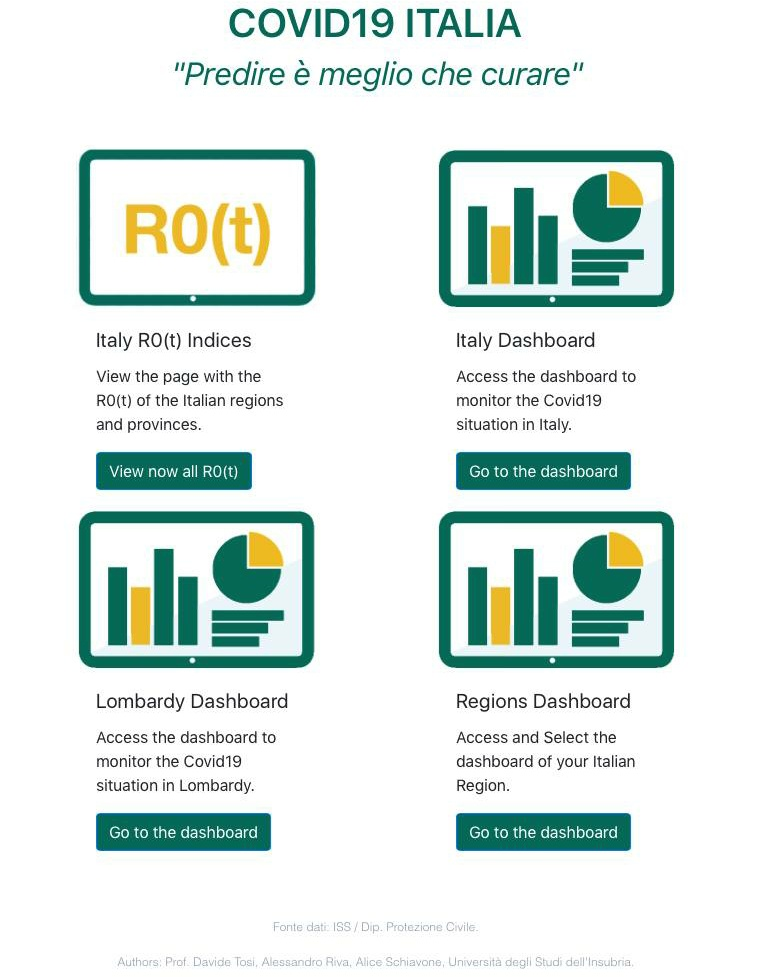
\includegraphics[width=15cm]{covid_19_italy_compact}
    \caption{Pagina principale del sito}
    \label{fig:home_page}
\end{figure}
\begin{figure}[htp]
    \centering
    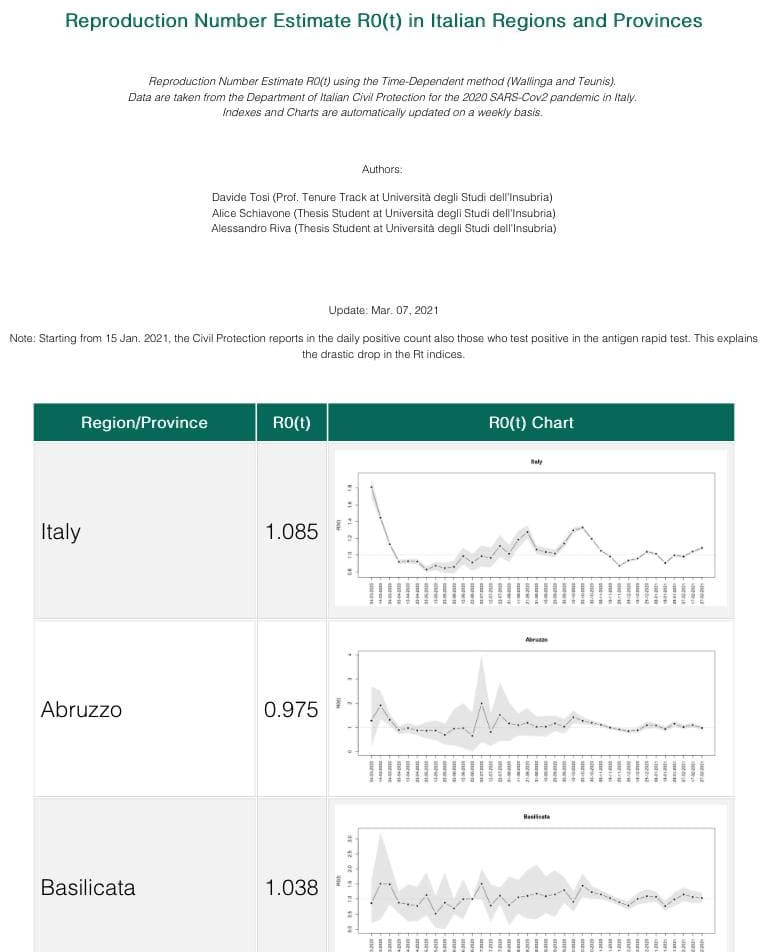
\includegraphics[width=15cm]{img/r0_screen.jpg}
    \caption{Pagina degli indici R0(t)}
    \label{fig:indici_r0}
\end{figure}

\section{Rassegna stampa}
Sono stati pubblicati numerosi articoli riguardanti il portale \emph{Covid19-italy.it}.\\
Alcuni sono riportati di seguito in ordine cronologico.\\

29 ottobre 2020: 
\begin{itemize}
    \item \emph{Covid: online nuovo portale grafici indice R0 in Lombardia}\cite{covid19-italy_ansa}
    \item \emph{La pandemia spiegata con numeri e grafici nel portale dell’Insubria}\cite{covid19-italy_varesenews}
\end{itemize}
14 novembre 2020:
\begin{itemize}
    \item \emph{Covid: "La discesa dei contagi inizierà a dicembre"}\cite{discesa_contagi_giorno}
\end{itemize}
19 novembre 2020:
\begin{itemize}
    \item \emph{Covid, Davide Tosi (Insubria) e Massimo Galli insieme per la divulgazione scientifica}\cite{covid_corriere_como}
\end{itemize}
14 febbraio 2021
\begin{itemize}
    \item \emph{"Ho raccontato il Covid con i numeri. Che non mentono mai"}\cite{raccontato_covid_ilgiorno}
\end{itemize}
\newpage
\section{Statistiche}
Il portale \emph{covid19-italy.it} ha riscosso sin da subito un discreto successo, sono stati registrati mediamente 200 utenti attivi al giorno per un totale di quasi 19.000 visitatori, nel periodo compreso tra la fine di settembre 2020 e l'inizio di marzo 2021.

\begin{figure}[htp]
    \centering
    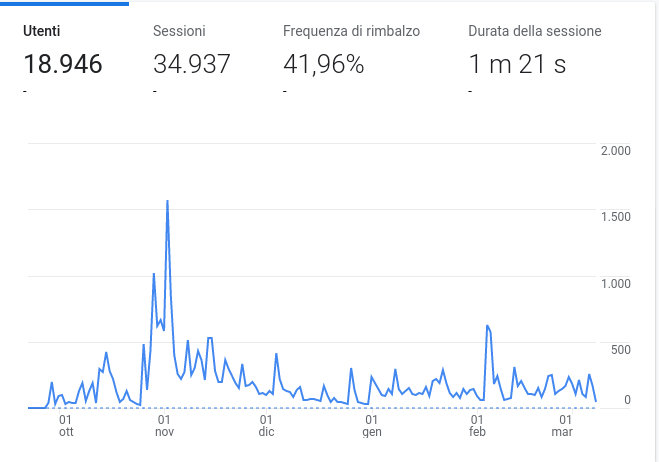
\includegraphics[width=10cm]{img/analytics.png}
    \caption{Statistiche da Google Analytics}
    \label{fig:statistics}
\end{figure}
